\subsection{センターコンピュータ}
\par ロボットの制御用センターコンピュータの構成について以下にまとめる.
\subsubsection{制御用PC}
\par ロボットの制御にはラップトップPCを使用した.CPUはインテル製Core m5(1.10GHz)を搭載しており,OSはUbuntu 14.04LTSを使用した.また,ロボット制御用のミドルウェアとしてROS(Robot Operating System)を使用した.
\subsubsection{モータドライバ}

\par モータドライバはCytron Technologies製 2ch DCブラシモータドライバ MDD10A(Fig.\ref{MDD10A})
を使用した.本製品はPWM信号を入力することにより速度制御を行うことができる.
\par ロジック電圧は5[V]であり,後述のモータコントローラを介してPCから給電される.

\begin{figure}[hb]
	\centering
	\includegraphics[clip,scale=0.08]{./figure/MDD10A.eps}
	\caption{MDD10A}
	\label{MDD10A}
\end{figure}
\newpage
\subsubsection{モータコントローラ}
\par エンコーダパルスカウンタおよびモータコントローラには iXs Research製 超小型USB接続4chモータコントローラ iMCs01(Fig.\ref{iMCs01})を使用した.本製品は最大3組のエンコーダ・DCモータの制御が可能である.また,入力には2相エンコーダ入力信号(4000pps未満),出力はPWM信号・CW/CCWが利用可能である.さらに,USBでPCから直接制御することが可能かつ,内部にPID制御式(\ref{imcs_eq})を持っているためにプログラム上でゲインの設定を行うだけで用意に制御が可能である.
制御出力 u は次式から 1[ms]毎に計算される.

\begin{eqnarray}
	u=A-\frac{K_P}{K_{P_x}}(v_d - v)%-\frac{K_D}{K_{D_x}}(\dot v_d - \dot x)
	-\frac{K_I}{K_{I_v}}\sum_0^t (v_d-v)
\label{imcs_eq}
\end{eqnarray}

このとき,Aはオフセットであり,$K_P・K_I$はそれぞれ比例・積分ゲインである.また,$v_d$は目標速度,$v$は現在値である.\\
\par ただし,本モータコントローラは本来位置制御に特化したものであるので現在値を得る際には,
\begin{equation}
	v = \frac{x_i - x_{i-1}}{t}
\end{equation}
から求める.このとき$x_i$は現在位置, $x_{i-1}$は1ステップ前の位置であり,$t$は1ステップの時間である.

\begin{figure}[hb]
	\centering
	\includegraphics[clip,scale=0.06]{./figure/IMCS01.eps}
	\caption{iMCs01}
	\label{iMCs01}
\end{figure}

% \subsubsection{電源}
% 石川鉄鋼所にきかなければー
%--------------------------------------------------------------------------------------------------
\newpage
\subsection{汎用フレーム} \label{frame}
\par 本研究で開発する移動ロボットには,駆動モジュールの増減に合わせて走行アルゴリズムを2輪・4輪・6輪と変更できるような汎用性が求められる.そこで,フレームの形状をFig.\ref{geneframe_fig}のようなX字にすることで追加パーツを組込むだけで駆動モジュールの数を変更できるようにした.実際に製作したフレームがFig.\ref{geneframe_cmp}である.

\begin{figure}[hb]
	\centering
	\includegraphics[clip,scale=0.8]{./figure/geneframe_fig.eps}
	\caption{汎用フレーム 概念図}
	\label{geneframe_fig}
\end{figure}





%-------------------------------------------------------------------------------------------------- 
\newpage
\subsection{駆動モジュール} \label{module}
\subsubsection{駆動モジュール構成}
\par 駆動モジュールはDCモータ,ロータリエンコーダ,ホイールによって構成されている.概念図と実際に製作した駆動モジュールをFig.\ref{drivingmod}に示す.各部はギアによって伝達されており,モータとエンコーダのギア比は2:1,モータとホイールのギア比は1:2となっている.\\
\par また,\ref{DCmotor}で示すDCモータを使用した際にこのモジュールが出せる最高速は,$0.774$[m/s]である.このとき$D$は車輪の直径である.

\begin{eqnarray}
	Vel_{max}  &=&\frac{rpm}{60sec}\cdot \pi \cdot	D\\ \nonumber
	 &=&\frac{98.5}{60}\cdot \pi \cdot 0.15 = 0.774
\end{eqnarray}

\begin{figure}[ht]
	\centering
	\begin{tabular}{cc}

		\begin{minipage}{0.5\hsize}
		\centering
		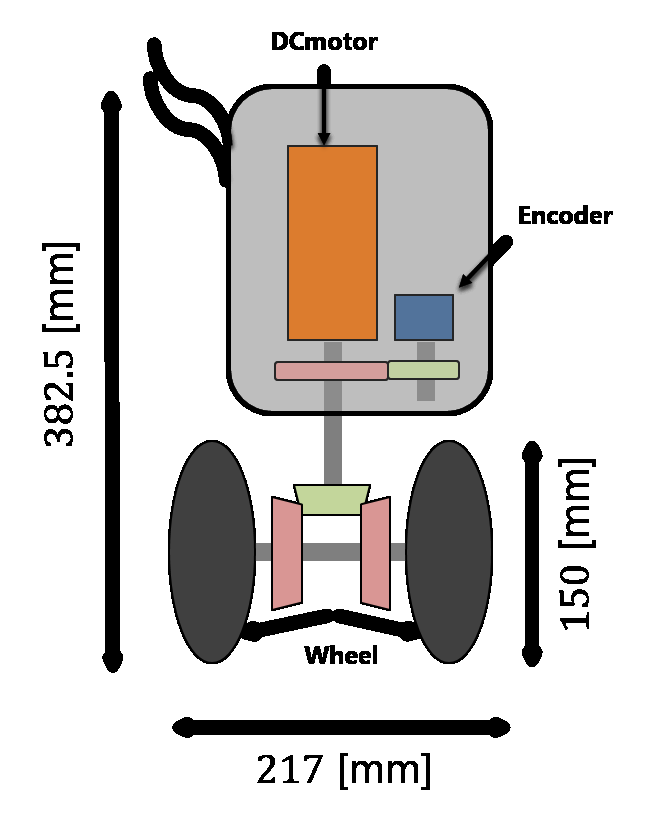
\includegraphics[clip,scale=0.5]{./figure/drivingmod_fig.eps}
		\hspace{1.6cm}
		\caption{概念図}
		\end{minipage}

		\begin{minipage}{0.5\hsize}
		\centering
		\includegraphics[clip,scale=0.06,angle=270]{./figure/driving_mod.eps}
		\hspace{1.6cm}
		\caption{製作した駆動モジュール}
		\end{minipage}

	\end{tabular}	
	\caption{駆動モジュール}
	\label{drivingmod}
\end{figure}
\newpage
\subsubsection{DCモータ}\label{DCmotor}
\par 各モジュールは駆動用としてそれぞれDCモータを搭載している.モータには,シンクエンジニアリング製 TE-38F16-24-64(Fig.\ref{dc-motor})使用した.モータ仕様をTab.\ref{motor_spec}に示す.

\begin{figure}[hb]
	\centering
	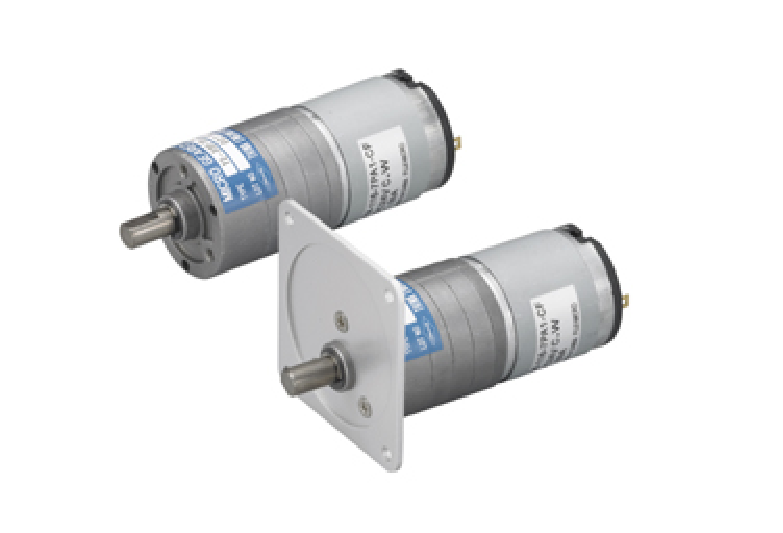
\includegraphics[clip,scale=0.6]{./figure/te-38f16-24-64.eps}
	\caption{DCモータ}
	\label{dc-motor}
\end{figure}

\begin{table}[hb]
	\centering
	\caption{DCモータ仕様}
	\begin{tabular}{|c|c|c|c|c|} \hline
		Rotation speed (rpm) & Torque(mN$\cdot$m) & Current (A) & Length (mm) & Weight (kg)  \\ \hline \hline
		98.5 & 1881.6 & 2.3 & 77.0 & 360.0 \\ \hline
	\end{tabular}
	\label{motor_spec}
\end{table}
\newpage
\subsubsection{ロータリエンコーダ}
\par 車輪回転速度制御用に,各駆動モジュールにはomron製インクリメンタル型ロータリエンコーダE6A2-CW3E(Fig.\ref{encoder_fig})を搭載している.仕様についてTab.\ref{encoder_spec}にまとめる.

\begin{figure}[hb]
	\centering
	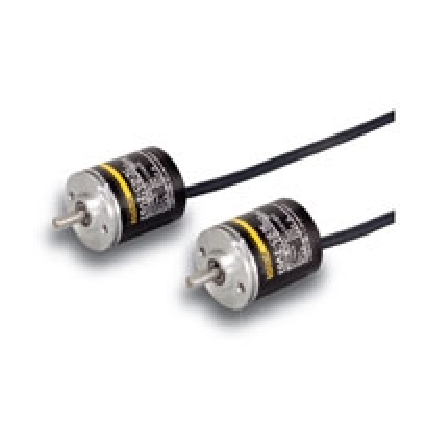
\includegraphics[clip,scale=1.0]{./figure/e6a2-c.eps}
	\caption{インクリメンタル型ロータリエンコーダ}
	\label{encoder_fig}
\end{figure}

\begin{table}[hb]
	\centering
	\caption{ロータリエンコーダ仕様}
	\begin{tabular}{|c|c|c|c|} \hline
		Power-supply (V),(mA) & Output phase & Output type & Maximum speed (rpm) \\ \hline \hline
		5-12,30 & A,B & Voltage & 5000 \\ \hline
	\end{tabular}
	\label{encoder_spec}
\end{table}
\newpage

%--------------------------------------------------------------------------------------------------
\subsection{3DLiDAR} \label{LiDAR}
\par 開発したロボットは環境を計測するための三次元計測センサとして,北陽電機社製3DLiDAR YVT-35LXを搭載している(Fig.\ref{yvt-35lx}).YVT-35LXの主なスペックをTab.\ref{yvt_spec}に示す.


\begin{figure}[hb]
	\centering
	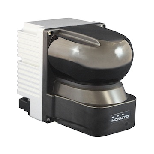
\includegraphics[clip,scale=2.5]{./figure/yvt-35lx.eps}
	\caption{3D LiDAR YVT-35LX}
	\label{yvt-35lx}
\end{figure}

\begin{table}[hb]
	\centering
	\caption{3D LiDAR YVT-35LX 仕様}
	\begin{tabular}{|c|c|} \hline
	& Specification \\ \hline
	Power 				& 10-30 [V](DC) \\ \hline
	Horizontal scan angle	& 210 [deg] \\ \hline
	Horizontal scan speed	& 20 [Hx]	\\ \hline
	Vertical scan angle		& 40 [deg](-5 - 35 [deg]) \\ \hline
	Vertical scan speed		& 1200 [Hz]	\\ \hline
						& 0.3-35 [m]($\-45<\theta < 45 $[deg]) \\
	Sensing distance	& 0.3-20 [m]($\-75 < \theta < -45,45<\theta<75$[deg]) \\
 						& 0.3-10 [m]($\theta< -75,75< \theta$[deg]) \\ \hline
	Accuracy			& $\pm$ 50 [mm](less than15[m]),$\pm$100[mm](than 15[m])\\ \hline
	Points of data		& 2590[points/frame] (20[fps])	\\ \hline
	Interface			& Ethernet(TCP/IP)				\\ \hline
	Weighy				& about 650[g]	\\ \hline
	Size				& 70[mm]$\times$106[mm]$\times$95[mm](W$\times$D$\times$H)\\ \hline
	\end{tabular}
	\label{yvt_spec}
\end{table}
%-----------------------------------------------------------------------------------
\newpage
\subsection{システム全体構成}
\subsubsection{ハードウェア構成}
\par ハードウェアの接続および構成についてFig.\ref{mod_sys_fig}に示す.また,完成した機体をFig.\ref{mod_robot_comp}に示す.

\begin{figure}[b]
	\centering
	\includegraphics[clip,scale=0.8]{./figure/mod_sys.eps}
	\caption{システム全体構成図}
	\label{mod_sys_fig}
\end{figure}

\subsubsection{ソフトウェア構成}
\par 